
\documentclass[
  master,
  program=ainfvs,
%  printversion,
  biblatex,
%  language=english,
%  font=sans,
  figures=true,
  tables=false,
%  theorems,
  sourcecodes,
  glossaries,
  index
]{kidiplom}


\title{Generátor logických her}
\title[english]{Logic game generator}


\author{Martin Hradílek}

\supervisor{doc. RNDr. Miroslav Kolařík, Ph.D.}

\yearofsubmit{\the\year}


\annotation{anotace}

\annotation[english]{annotation}

\keywords{logické hry; diplomová práce; sudoku; mosty; bludiště; zpětné vyhledávání; determinismus; }
\keywords[english]{logic games; master thesis; sudoku; bridges; mazes; backtracking; determinism; }

\thanks{Děkuji, děkuji, děkuji.}
\bibliography{bibliografie.bib}

\graphicspath{ {img/} }
\usepackage{lipsum}
\usepackage{longtable}
\usepackage{graphics}
\usepackage{amsmath}
\usepackage{listings}

\begin{document}

\maketitle

\section{Úvod}

\section{Teoretická část}

\subsection{Sudoku}

Sudoku je logická hra využívající čísla jako symboly, ale nevyžaduje žádné matematické operace. Základní verze Sudoku se hraje na čtvercové mřížce o velikosti $9 \times 9$, která je dále rozdělena do devíti menších čtvercových bloků (tzv. bloků) o rozměru $3 \times 3$.

Cílem hry je doplnit všechna prázdná pole čísly od 1 do 9 tak, aby se neopakovaly na žádném řádku, sloupci a bloku.
 
Na začátku hry je část polí již předvyplněna. Tyto pole slouží jako vodítko pro řešení a částečně určují obtížnost úlohy (více popsáno v podkapitole \ref{tacticsSubsection}).

Sudoku, jež můžeme označit jako validní, má 1 možné řešení. 
 

\begin{figure}[!htb]
	\centering
	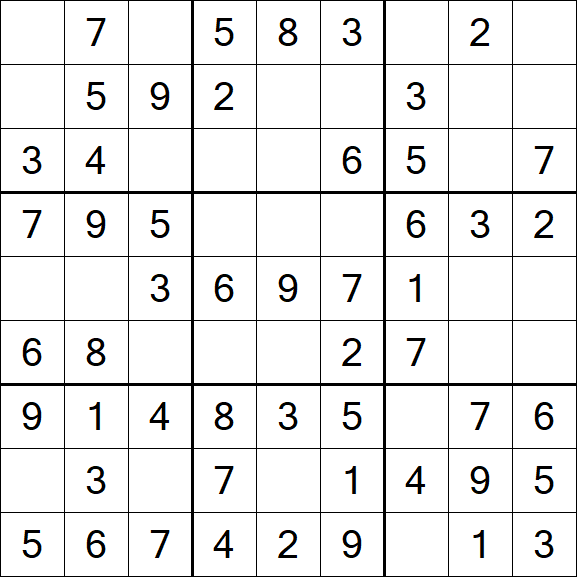
\includegraphics[height=5cm]{/sudoku/standard_sudoku.png}
	\caption[Sudoku 9x9]{Sudoku 9x9~\cite{CrossA2025}}
	\label{sudoku_9}
\end{figure}


\subsubsection{Historie}

Historie Sudoku se datuje až do 18. století. Sudoku v dnešní podobě bylo poprvé publikováno v magazínu Dell Pencil Puzzles and Word Games pod názvem Number Place. Hra se následně rozšířila do Japonska, kde získala svůj současný název Sudoku, což je zkrácenina japonského výrazu „Sūji wa dokushin ni kagiru“, což znamená: „Číslice jsou omezeny na jedno použití.“ \cite{Sudoku.com2025}

\subsubsection{Sudoku matematicky}

Základní problém Sudoku lze popsat jako kombinatorickou úlohu. Cílem je doplnit čtvercovou mřížku o rozměrech $n \times n$, rozdělenou do $k \times k$ bloků tak, aby v každém řádku, sloupci a bloku byly právě jednou použity všechny symboly z dané množiny velikosti n.

Obecný problém řešení Sudoku o rozměrech $n^2 \times n^2$, kde je mřížka rozdělena do $n \times n$ bloků, je známý jako NP-úplný problém \cite{Yato2003}.

Počet možností, jak lze sestavit hrací pole sudoku $9 \times 9$ je 6 670 903 752 021 072 936 960, tj. přibližně  $6.67 \times 10^{21}$ \cite{Felgenhauer2005}.

\subsubsection{Obtížnost a taktiky řešení}
\label{tacticsSubsection}

\subsubsection{Varianty Sudoku}

Mimo klasického $9 \times 9$ sudoku existuje mnoho verzí s jinými pravidly a limitacemi. Následující výčet a obrázky byly převzány z \cite{sudoku-puzzles.net}.

\begin{itemize}
	\item \textbf{Sudoku 4×4, 6×6 a další} – různé velikosti herní plochy, které vyžadují úpravu pravidel a používaných symbolů (např. A–F u 16×16)

	\begin{figure}[!htb]
		\centering
		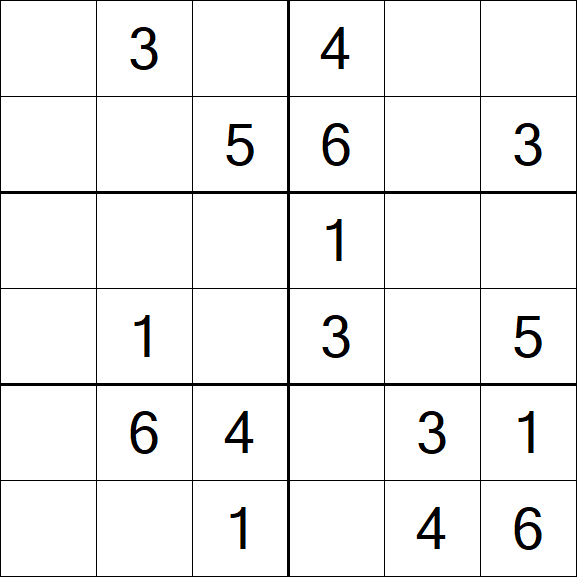
\includegraphics[height=5cm]{/sudoku/sudoku_6.png}
		\caption[Sudoku 6x6]{Sudoku 6x6}
		\label{sudoku_6}
	\end{figure}
	
	\item \textbf{Jigsaw Sudoku} – místo klasických čtvercových bloků $3 \times 3$ jsou bloky nepravidelné, ale stále musí obsahovat všechna čísla. Tato varianta je často kombinována s různými velikostmi herních ploch
	
	\begin{figure}[!htb]
		\centering
		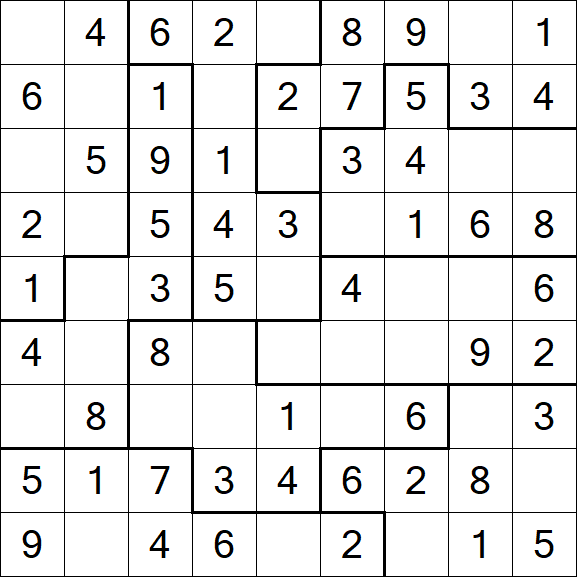
\includegraphics[height=5cm]{/sudoku/jigsaw_sudoku.png}
		\caption[Jigsaw Sudoku]{Jigsaw Sudoku}
		\label{sudoku_jigsaw}
	\end{figure}
	
	\item \textbf{Killer Sudoku} – přidává další pravidla ve formě klecí s hodnotou, ve kterých musí být společná hodnota čísel v nich rovna hodnotě klece
	
		\begin{figure}[!htb]
		\centering
		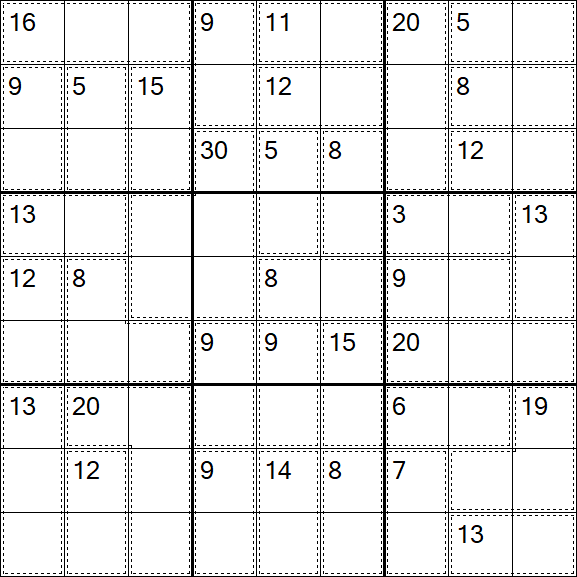
\includegraphics[height=5cm]{/sudoku/killer_sudoku.png}
		\caption[Killer sudoku]{Killer sudoku}
		\label{sudoku_killer}
	\end{figure}
	
	\item \textbf{Sudoku-DG} – Buňky jsou mimo stávající rozdělení rozčleněny do barevně označených skupin a platí, že v každé skupině (barvě) se čísla nesmí opakovat
	
	\begin{figure}[!htb]
		\centering
		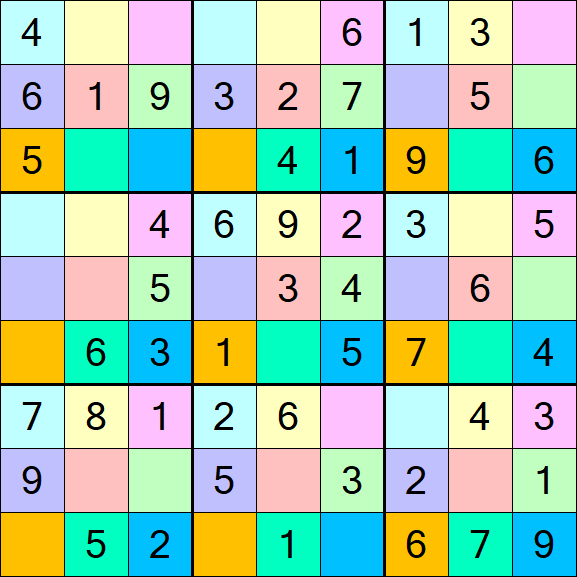
\includegraphics[height=5cm]{/sudoku/sudokuDG.png}
		\caption[Sudoku DG]{Sudoku DG}
		\label{sudoku_DG}
	\end{figure}
	
	\newpage
	\item \textbf{Samurai sudoku} – Hrací plocha je složena z pěti do sebe zapadajících $9 \times 9$ hracích ploch, kde centrální je překryta dalšími čtyřmi, přičemž sdílí v každém rohu $3 \times 3$ blok.
	
		\begin{figure}[!htb]
		\centering
		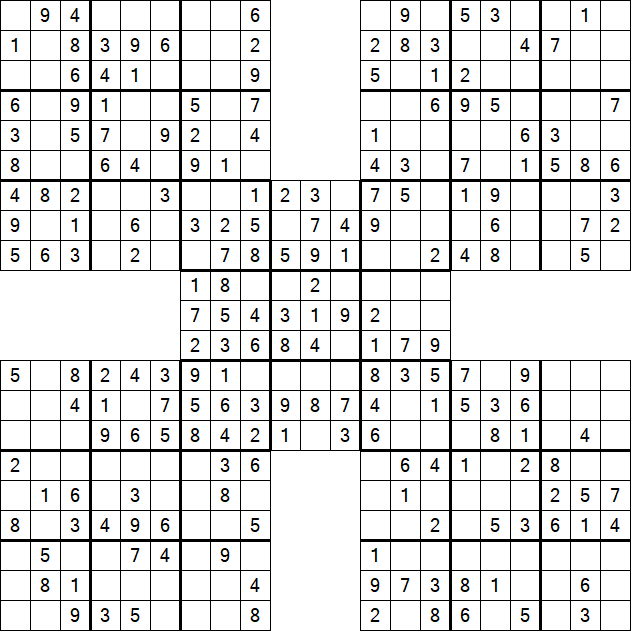
\includegraphics[height=7cm]{/sudoku/samurai_sudoku.png}
		\caption[Samurai Sudoku]{Samurai Sudoku}
		\label{sudoku_samurai}
	\end{figure}
\end{itemize}

Jigsaw Sudoku a různé velikosti hrací plochy jsou více popsány v \ref{implementedSudokuTypes}, kde je také pojednáváno o jejich implementaci.

\subsection{Mosty}

\subsection{Bludiště}

\section{Programátorská část}

\subsection{Sudoku}

\subsubsection{Implementované typy}
\label{implementedSudokuTypes}

\subsubsection{Vytvoření vyřešeného sudoku}

\subsubsection{Odstranění čísel v sudoku}

\section{Uživatelská část}

\begin{kiconclusions}

\end{kiconclusions}

\begin{kiconclusions}[english]
	
\end{kiconclusions}

\printglossary

\printbibliography

.
\printindex

\end{document}

%%% Local Variables:
%%% mode: latex
%%% TeX-master: t
%%% End:
